
\subsection{Hardware Test}

The functionality of the behaviours implemented can be tested individually.
Nevertheless, a more robust way of testing the behaviours is to combine them in certain test circuits that can be looped to check the reliability of these behaviours.
By building a more complex test circuit, the different behaviours can be tested in different ways so the position of the robot changes before each of them.

This way, three different experiments were conducted to test the reliability of the robot:

\begin{enumerate}
	\item First, a test to check the robot is able to find, follow and get a good position on a line after right and left turning. 
With this test we can test the follow line, and turning behaviours.
The circuit used in this test was a "8", that means, the robot should turn left four times and then right four times in a row
.

	\item The second test looks at the ability of the robot to go back in a intersection and turn to different directions after finding the previous intersection.
This test has the robot going in loops where it goes back, finds the next intersection and goes back again to the previous one. 
Then the robot turns in different directions each time, checking the response of all of them in different cases, as these directions are mixed.

	\item Finally, a experiment with a can was conducted to test the robots ability to push and place correctly the can.
In this experiment, the robot has to use all the different behaviours to move the can from one position to another and then to the original position again.

\end{enumerate}

The circuits used in each experiments are shown in the figure \ref{fig:testMaps}

All of the three experiments were started with a fully charged battery and the test was repeated 20 times in up to 10 trials without a battery change or charge.
The time needed to complete the 20 laps was measured for each trial.
This makes it possible to determine the functionality and response of the robot in long runs.
The result of such is seen in table \ref{tab:Experiment1}.

The light sensors response to different ambient light levels was tested and the shielding was found to protect the sensors efficiently.
Furthermore the can was still able to pass through the shielding added in the front of the robot for when the robot drives towards a light source.
%The information about this research is attached in \textbf{reftolightsensors}.


\begin{figure}[H]
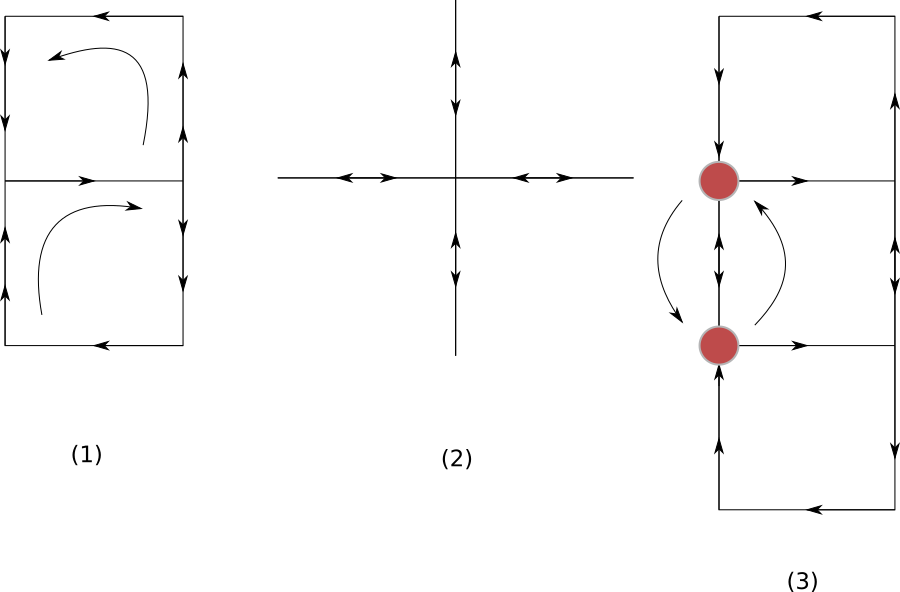
\includegraphics[width=10cm]{Test_circuits.png}
\centering
\caption[Behaviours used for testing.]{Scheme of the circuits used in the tests. 1, loop for turning behaviours. 2, used for pushing and going back behaviours. 3, used for testing the pushing behaviour with a can. }
\label{fig:testMaps}
\end{figure}


\subsection{Results}
	The results of the tests in table \ref{tab:Experiment1} show that the chosen configuration is robust enough to complete any sokoban map.
	All the behaviours have been tested and work for all the test or just a period of time, after which they then fail mainly because of low battery.
	%, as the failures start when the robot has been running for a long time.
	This happens when doing the pushing and going back behaviour, which means this is the weakest part of the implementation.
	Nevertheless, the number of failures of this behaviour is small enough to be ignored.
This is because the time spent running without battery charge has been above the 30 minutes in all experiments and it can be assumed that the robot will not have power problems during its operating time, which is of 15 minutes at max during the competition.
	
	
	Finally, it is possible to say that the robot configuration is robust under different light levels due to the used shield.
	Furthermore the robot control is able to complete the map.


\begin{table}[H]
	\center
	
	\begin{tabular}{|l|c|r|c|r|c|r|}
	  	\cline{2-7}
	  	\multicolumn{1}{r}{}
 		&  \multicolumn{2}{|c|}{Map 1}
 		& \multicolumn{2}{|c|}{Map 2} 
 		& \multicolumn{2}{|c|}{Map 3}  
		 \\ \cline{2-7}
		\hline
		Run & Success & Time & Success & Time & Success & time \\
		\hline
		1 	& Yes & 6'26'' & Yes & 5'28'' & Yes & 8'16''\\
		2 	& Yes & 6'21'' & Yes & 5'33'' & Yes & 8'15''\\
		3 	& Yes & 6'27'' & Yes & 5'29'' & Yes & 8'17''\\
		4 	& Yes & 6'29'' & Yes & 5'30'' & Yes & 8'05''\\
		5 	& Yes & 6'33'' & Yes & 5'31'' & Yes & 8'15''\\
		6 	& Yes & 6'33'' & No  & 5'10'' & Yes & 8'10''\\
		7 	& Yes & 6'55'' & Yes & 5'34'' & Yes & 8'25''\\
		8 	& Yes & 6'52'' & Yes & 5'41'' & Yes & 8'54''\\
		9 	& No & LOWBAT  & No  & 1'13'' & No 	& LOWBAT\\
		10 	& No & LOWBAT  & No  & 1'50'' & No 	& LOWBAT\\		
		\hline
	\end{tabular}

	\caption[Experimental results of the robot behaviour.]{Results of the experiments. It is shown for each experiment and result the success or failure of the test and the time used on completing it. In the case of the failed trials, the time shown represents the moment when the robot was lost. The LOWBAT statement means the robot finished his power and the experiment finished.}
	\label{tab:Experiment1}
\end{table}